\documentclass{article}

% Language setting
% Replace `english' with e.g. `spanish' to change the document language
\usepackage[english]{babel}
\usepackage[table]{xcolor}
\usepackage{graphicx,caption}
% Set page size and margins
% Replace `letterpaper' with`a4paper' for UK/EU standard size
\usepackage[letterpaper,top=2cm,bottom=2cm,left=3cm,right=3cm,marginparwidth=1.75cm]{geometry}
\usepackage{nicematrix}
\usepackage{tikz}
\usetikzlibrary{patterns}
\usetikzlibrary {patterns.meta}
\pgfdeclarepattern{
  name=hatch,
  parameters={\hatchsize,\hatchangle,\hatchlinewidth},
  bottom left={\pgfpoint{-.1pt}{-.1pt}},
  top right={\pgfpoint{\hatchsize+.1pt}{\hatchsize+.1pt}},
  tile size={\pgfpoint{\hatchsize}{\hatchsize}},
  tile transformation={\pgftransformrotate{\hatchangle}},
  code={
    \pgfsetlinewidth{\hatchlinewidth}
    \pgfpathmoveto{\pgfpoint{-.1pt}{-.1pt}}
    \pgfpathlineto{\pgfpoint{\hatchsize+.1pt}{\hatchsize+.1pt}}
    \pgfpathmoveto{\pgfpoint{-.1pt}{\hatchsize+.1pt}}
    \pgfpathlineto{\pgfpoint{\hatchsize+.1pt}{-.1pt}}
    \pgfusepath{stroke}
  }
}

\tikzset{
  hatch size/.store in=\hatchsize,
  hatch angle/.store in=\hatchangle,
  hatch line width/.store in=\hatchlinewidth,
  hatch size=5pt,
  hatch angle=0pt,
  hatch line width=.5pt,
}

\newcommand{\MyBlock}{\Block[tikz={pattern=hatch, pattern color=gray, hatch size=2pt}]}




\definecolor{royalblue(web)}{rgb}{0.25, 0.41, 0.88}

\usepackage{amsmath}
\usepackage[colorlinks=true, allcolors=blue]{hyperref}

\title{Liste des projets}
\date{}
\begin{document}
\maketitle

\vspace{2cm}


\vspace{2cm}
{\large
\textbf{Branche BMC-SAT} : \url{https://github.com/Dowsers/Dowsers_Solution/tree/ak/bmc} \\
  
\textbf{Branche SMARTPULSE} : \url{https://github.com/Dowsers/Dowsers_Solution/tree/ak/smartpulse}\\


\textbf{Branche HLL-SMT2} : \url{https://github.com/ssie2025-pfe2/hll2smt-py}\\

  
}
\newpage
\section{Bounded model checking par le SAT}

\begin{figure}[h]
    \hspace{-0.8cm}
    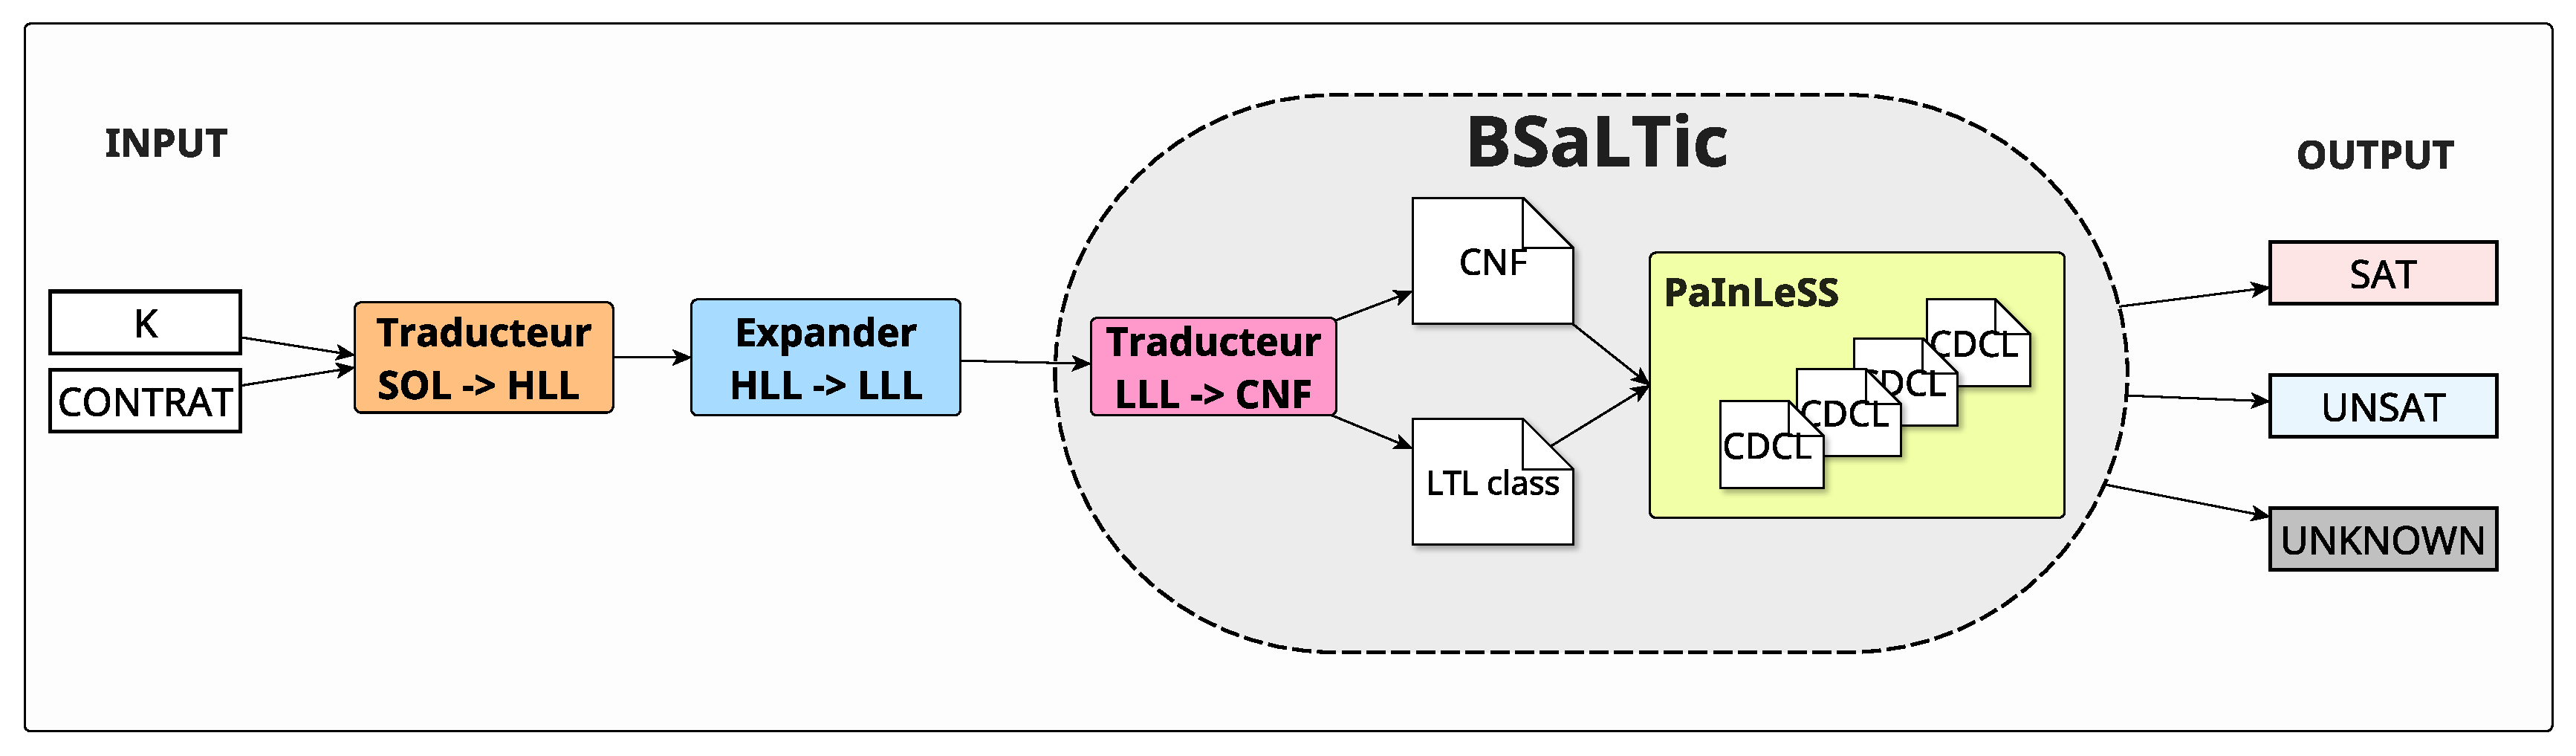
\includegraphics[scale=0.28]{bsaltic_framework_solidity.pdf}
    \caption{BMC-SAT architecture}
    \label{fig:bmcsat}
\end{figure}
\subsection{Contexte}


Le model checking~\cite{modelchecking} peut fournir un contre-exemple (CEX) lorsqu'un modèle ne satisfait pas une exigence (spécification). Ce CEX correspond à un chemin d'exécution du système, ce qui aide considérablement les concepteurs à comprendre où se situe le problème dans le système.
%
Pour réaliser cette vérification, il est nécessaire d'effectuer une traversée complète de l'espace des états représentant les comportements du modèle. Deux approches ont été utilisées : le model-checking explicite et le model-checking symbolique.

Sur ce projet, nous nous concentrons sur les techniques symboliques qui utilisent des procédures de résolution SAT, devenues un pilier du model-checking moderne. 

En particulier, les procédures SAT sont largement utilisées dans la version \textit{bornée} du model-checking, notamment pour la vérification des spécifications LTL (Linear Temporal Logic). 

Le Bounded Model Checking (BMC)~\cite{bmcbiere,bmcsat,symbolicMC2} désigne une approche de model-checking  où la vérification de la propriété est effectuée à l'aide d'une traversée limitée, c'est-à-dire une traversée d'une représentation symbolique de l'espace d'états qui est bornée par un entier $k$. Cette approche ne nécessite pas le stockage de l'ensemble de l'espace d'états, ce qui la rend plus souple et utile.
%~\cite{improveSATBMC,satbasedMC}.



Les solveurs SAT modernes sont ainsi devenus la technologie centrale de nombreux model checkers. Cette
%
Leurs efficacité est principalement due aux nombreuses optimisations qui ont été développées pour orienter les procédures SAT vers des espaces de recherche prometteurs, réduisant ainsi les temps de résolution. Une optimisation particulièrement remarquable implique la génération et l'utilisation d'informations de haute qualité (apprentissage) provenant des solveurs SAT, à base d'apprentissage par conflit~\cite{grasp,MoskewiczMZZM01} (Conflict Driven Clause Learning algorithm, CDCL), ce qui permet l'élagage de sous-espaces inutiles.

\subsection{Branche BMC-SAT}
\hspace{0.5cm}-- \textbf{Dépôt} : \url{https://github.com/Dowsers/Dowsers_Solution/tree/ak/bmc} \\
  
  -- \textbf{Objectif} :  (1) Vérifier la fiabilité d'un Smart Contract sur une propriétés, passe par la résolution de la formule SAT qui les traduit. La vérification est limitée à nombre de transactions $k$ défini au préalable. 
  
  \hspace{2.1cm}(2) Étudier les informations importantes à sauvegarder lors de la phase d'apprentissage par conflit du SAT solveur CDCL. Ainsi, pouvoir adapter les heuristiques de stockage d'information selon les caractéristiques des contrats Solidity.  \\

-- \textbf{Entrée} : (1) Solidity Smart Contract version \textbf{0.8.x}, 

\hspace{1.72cm} (2) nombre de transactions $k$.\\

-- \textbf{Sortie} : \{CEX, OK, UNKNOWN\} où CEX signifie que la propriété est invalide, OK elle est vérifiée et UNKNOWN si non décidé.\\

-- \textbf{Langage pivot}: HLL


\subsection{Calendrier}

\textbf{Avril-Juillet} :

 • Optimisation du convertisseur LLL vers le format d'entrée du SAT solveur (Forme Normale Conjonctive, CNF).
 
 • Intégration d'un SAT solveur récent KISSAT-MAB~\cite{kissat-mab} (gagnant de la compétition 2022).
 
 • Adaptation des heuristiques de stockage d'information du SAT solveur pour les contrats Solidity.
 
 • Expérimentation et comparaison de l'approche BMC-SAT avec l'existant (résolution par induction \textit{PROVER}).

\hspace{-0.5cm}\\
\textbf{Octobre} :

 • Intégration complète de l'approche BMC-SAT avec le reste des techniques.
 
 • Intégration d'une version concurrente des stratégies de vérification existantes (BMC-SAT et PROVER) : un portefeuille de stratégies qui résolvent le même contrat avec les mêmes propriétés (dépôt \url{https://github.com/Dowsers/Tarkastus_Docker_AWS/tree/dev/portfolio})
 
 \hspace{-0.5cm}\\
\textbf{Novembre-Décembre} :

 • Amélioration du projet : techniques de parallélisation, partage d'information précises, ... 

\newpage

\section{Büchi contract}


\begin{figure}[h]
    \centering
    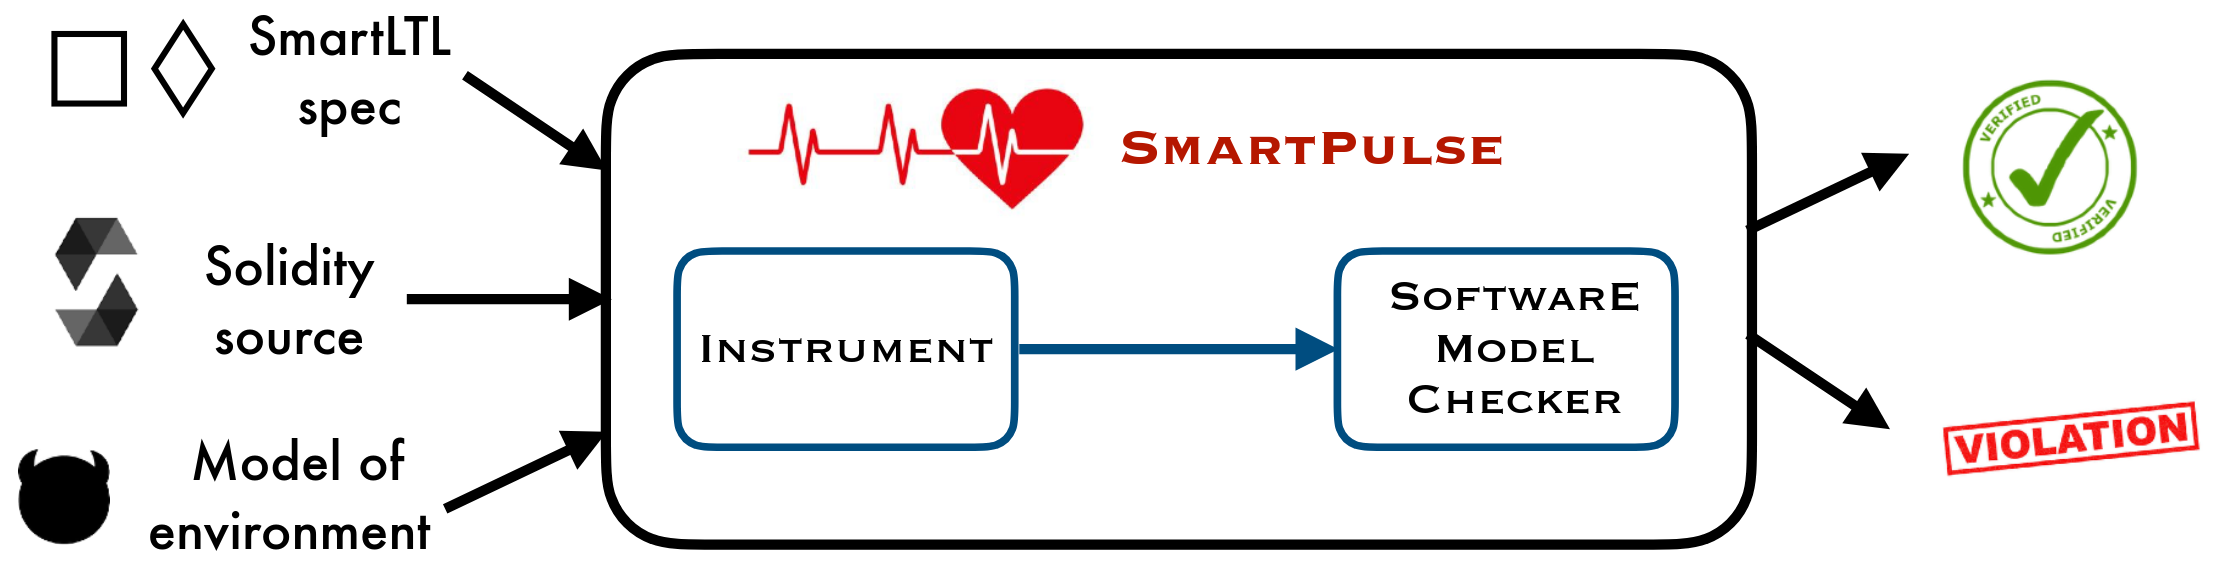
\includegraphics[scale=0.18]{smartpulse.png}
    \caption{SmartPulse architecture}
    \label{fig:smartpulse}
\end{figure}
\subsection{Contexte} 

Par Büchi contrat, nous entendons un smart contract accompagné de sa spécification représenté sous forme d'automate de Büchi.

Ce projet se focalise sur l'intégration de SmartPulse dans notre portefeuille de techniques de vérification. Produit par Microsoft employant des travaux de l'université de Freiburg, SmartPulse n'est plus maintenu depuis 2019.

L'outil repose sur trois principes de conception :

\begin{enumerate}
\item \textbf{Un langage de spécification ergonomique et expressif :} SmartPulse permet aux utilisateurs de spécifier leurs propriétés dans un langage appelé SmartLTL. SmartLTL est basé sur la logique temporelle linéaire (LTL), un formalisme (\textit{intuitif}) pour exprimer les propriétés des traces dans le temps. Cependant, SmartLTL étend la LTL standard avec des constructions supplémentaires qui facilitent l'expression des propriétés de correction des smart contracts. SmartPulse est ainsi capable de vérifier les propriétés de vivacité (liveness).


\item \textbf{Possibilité de personnaliser les modèles d'attaque :} SmartPulse est paramétré par un modèle d'environnement qui permet d'expérimenter différents modèles d'attaque. Par exemple, l'approche permet aux utilisateurs de personnaliser les hypothèses sur la façon dont l'attaquant peut interagir avec un contrat par le biais d'appels externes.

\item \textbf{Automatisation et précision :} SmartPulse est un outil entièrement automatisé basé sur le paradigme du raffinement de l'abstraction guidé par les contre-exemples (CEGAR) et fournit une approche unifiée pour la recherche simultanée de preuves et de violations à l'aide d'un solveur SMT (SAT modulo Theory)~\cite{BarFT-SMTLIB}. En outre, dans les cas où SmartPulse signale une erreur, il peut générer une attaque concrète dans laquelle la propriété sera violée. 

\end{enumerate}

\begin{flushleft}
Partant d'une spécification formelle rédigée en SmartLTL, d'un contrat Solidity et d'un modèle d'attaque, SmartPulse effectue d'abord une séquence d'instrumentations de programme pour modéliser l'environnement d'exécution du contrat et utilise ensuite une approche de vérification basée sur CEGAR pour rechercher des violations de propriétés (au travers d'automate de Büchi).

%SmartPulse offre un panel de méthodes de vérification : (a) model-checking implicite au travers des SAT solveur SMT (Sat Modulo Theory), (b) model-checking explicite au travers d'automates de büchi. Le comportement du modèle ainsi que la propriété sont représentés sous forme d'automates de Büchi pour le modèle et la propriété LTL~\cite{buchi1990,buchi1994}. Ensuite, un produit synchronisé (\textit{emptiness check}) est effectué. Si le produit est vide, la propriété est vérifiée ; sinon, elle est violée. %Le principal inconvénient de cette technique est le problème de l'explosion de l'espace d'états~\cite{statespaceexplosion}, ce qui signifie que la taille de l'espace d'états du système augmente de manière exponentielle.
\end{flushleft}


\subsection{Branche SMARTPULSE}

\hspace{0.5cm}-- \textbf{Dépôt} : \url{https://github.com/Dowsers/Dowsers_Solution/tree/ak/smartpulse}\\


-- \textbf{Objectif} : (1) S'approprier l'outil et le mettre à niveau (plusieurs expressions Solidity ne sont pas pris en compte : \textit{inline assembly, bitwise operations, fonctions ABI, etc}.

\hspace{2.05cm} (2) Intégrer la branche BMC-SAT dans SmartPulse.

\hspace{2.05cm} (3) Implémenter des techniques de model-checking explicite (\textit{emptiness check}).\\

\hspace{-0.5cm}-- \textbf{Entrée} : (1) Smart Contract Solidity version \textbf{0.5.10},

\hspace{1.25cm} (2) Spécification au format SmartLTL,

\hspace{1.25cm} (3) Model d'attaque \textit{(optionnel)}. \\

\hspace{-0.5cm}-- \textbf{Sortie} : \{CEX, OK, UNKNOWN\} \\

\hspace{-0.5cm}-- \textbf{Langage pivot} : Boogie (\textit{modifié})

\subsection{Calendrier}
\textbf{Septembre : }

 • Prise en main de l'outil \textit{non documenté}.
 
 • Difficultés d'installation de SmartPulse (packages obsolètes)
 
 • Mise à niveau de certains sous-outils/packages (VeriSol~\cite{wang2019formal}, Corral~\cite{lal2012corral}).

\hspace{0.5cm}\\
\textbf{Octobre :}

 • Création d'un docker pour faciliter l'utilisation de SmartPulse.
 
 • Temporairement et pour des objectifs d'expérimentation : création d'un script qui adapte des contrats Solidity \textbf{0.[5-8].x} en \textbf{0.5.10}.
 
 • Génération automatique des spécifications ERC20 en SmartLTL.\\

\hspace{-0.5cm}\textbf{Novembre-Décembre :}

 • Passage vers Solidity \textbf{0.8.x}

 • Comparaison de SmartPulse avec les outils de vérification existantes (BMC-SAT et PROVER).
 
 • Commencer l'optimisation des techniques de vérification de SmartPulse.

\newpage

\section{Convertisseur HLL vers SMT2}
\subsection{Contexte}

\begin{figure}[h]
\hspace{-1cm}
    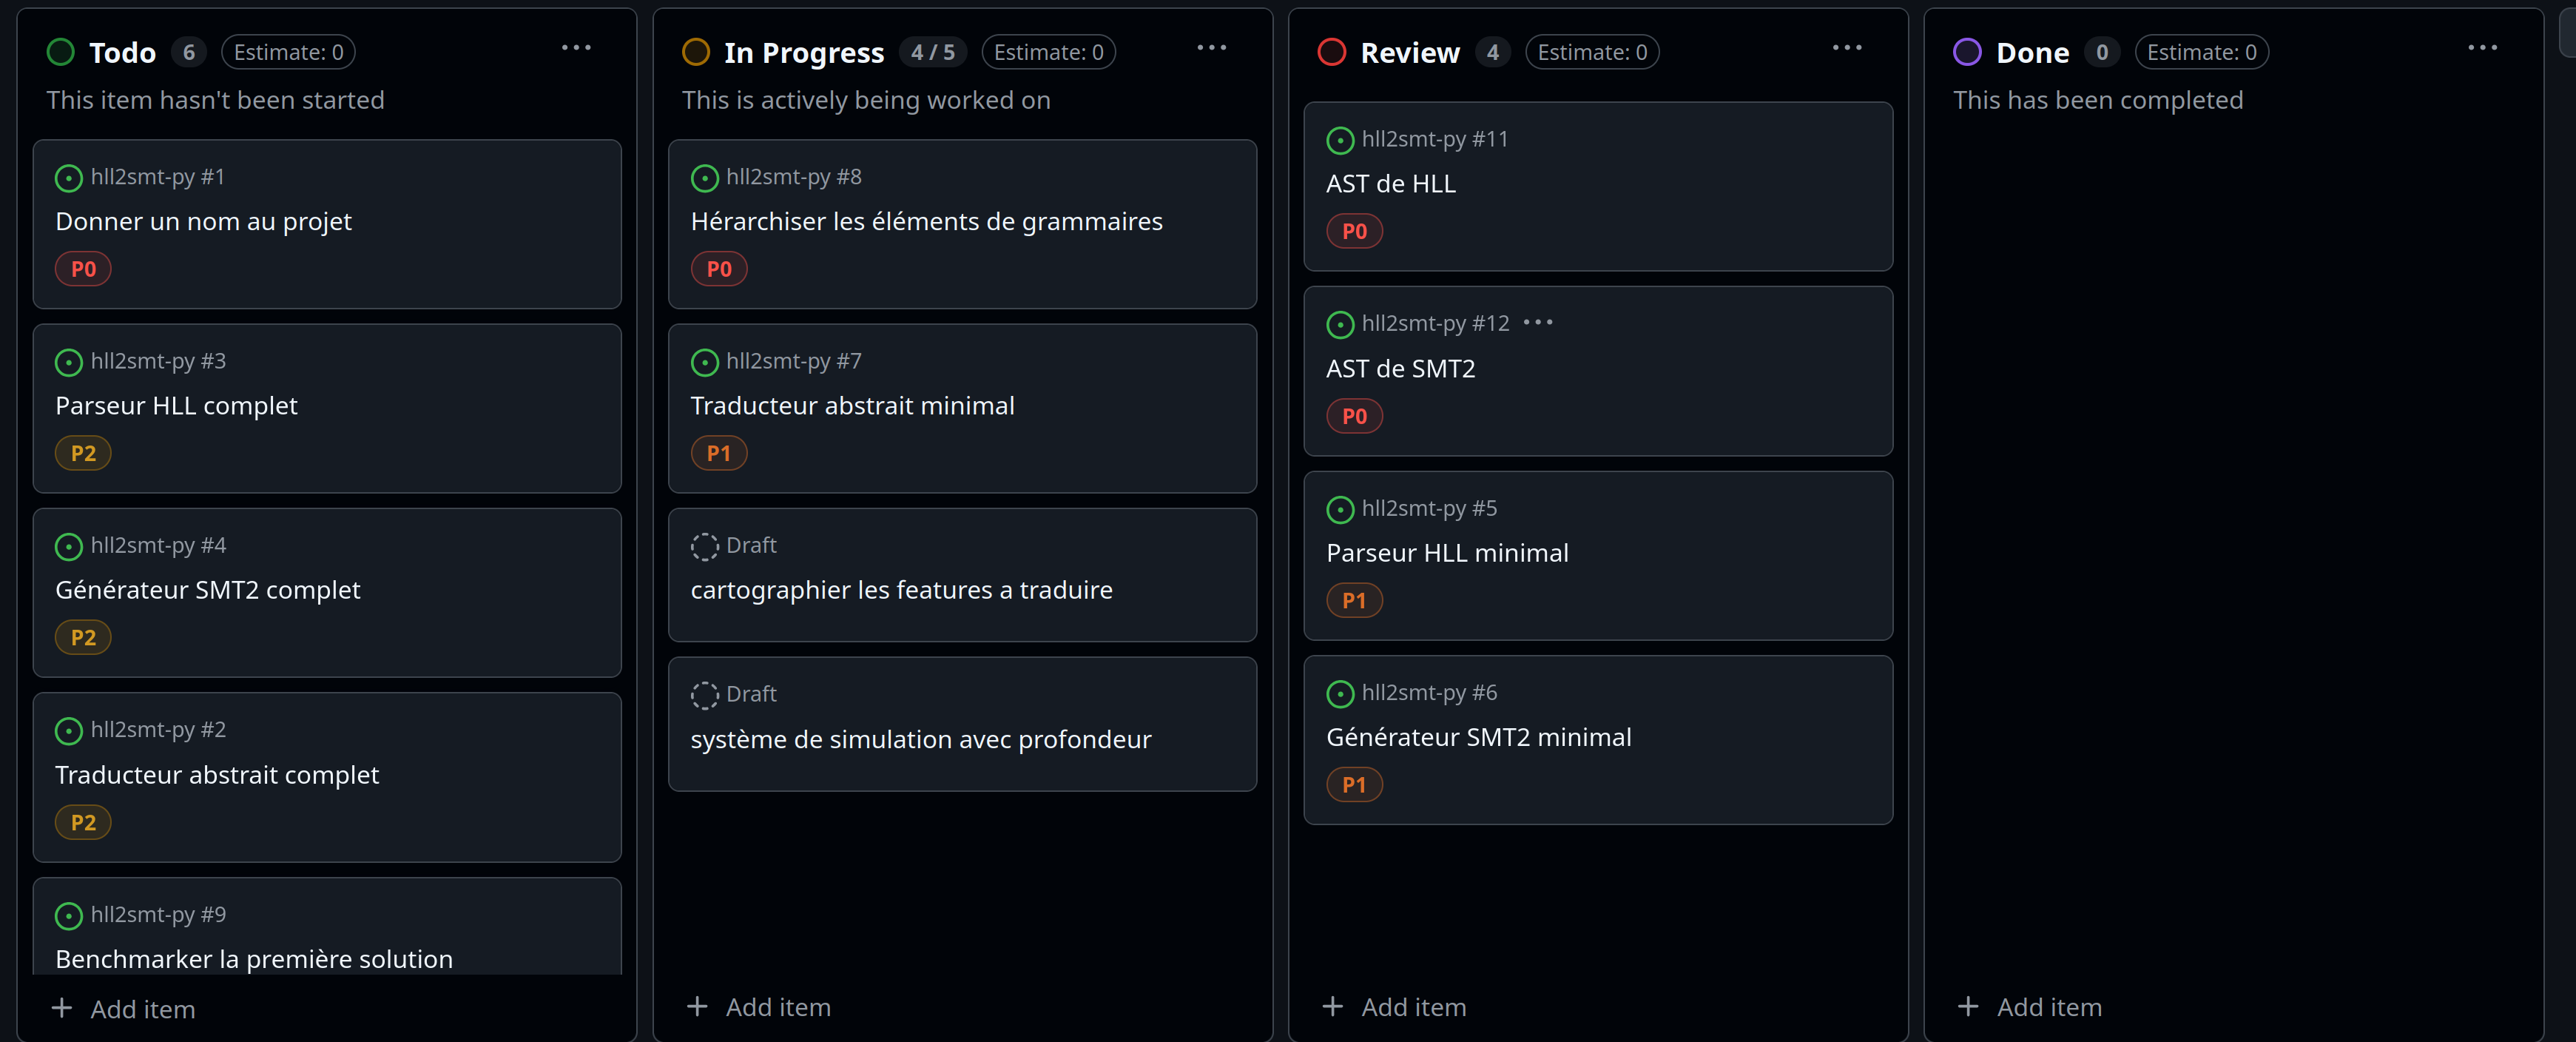
\includegraphics[scale=0.14]{avancement_pfe.png}
    \caption{Avancement projet HLL-SMT2}
    \label{fig:avancement}
\end{figure}

Ce projet est en cours de développement par les étudiants de EPITA Toulouse. Il vise à construire un traducteur du langage pivot HLL vers un problème SMT2.

Les SAT Modulo Theory (SMT)~\cite{BarFT-SMTLIB} sont des problèmes de décision pour des formules de logique du premier ordre avec égalité (sans quantificateurs), combinées à des théories dans lesquelles sont exprimées certains symboles de prédicat et/ou certaines fonctions (\textit{logique propositionnelle, arithmétique entiers et réels, bitvectors, arrays, dataType, floating points, string}).

%Fonctionnement de base d'un solveur SMT repose sur deux points : résolution par SAT solveur et une ou plusieurs procédures de décision de la théorie. 

%(1) Si pas de modèle SAT, la formule n’est pas satisfiable.\\
%(2) Si modèle SAT, vérification de la cohérence avec des procédures de décision de la théorie :
%    (a) Si cohérence, la formule est satisfiable
%    (b) Si pas cohérence, on cherche un autre modèle


\subsection{Branche HLL-SMT2}

\hspace{0.5cm}-- \textbf{Dépôt} : \url{https://github.com/ssie2025-pfe2/hll2smt-py}\\


-- \textbf{Objectif} : (1) Traduire n'importe quelle instance HLL au format SMT2.

\hspace{2.15cm}(2) Exploiter les approches de vérification formelle à base de solveur SMT.\\


-- \textbf{Entrée} : (1) Fichier au format HLL,

\hspace{1.75cm} (2) nombre de transactions $k$.\\

-- \textbf{Sortie} : Fichier au format SMT2.


\subsection{Calendrier}
La figure~\ref{fig:avancement} ci-dessus liste les avancés de ce projet.


\hspace{-0.5cm}\\
\textbf{Septembre-Octobre :}

• Finalisation des Arbres Syntaxiques Abstraites (AST) du langage HLL et SMT2.

• Première conversion d'une instance HLL à une variable accomplie.

• Hiérarchiser les éléments de grammaires.

• Cartographie des syntaxes et expressions à traduire.

\hspace{-0.5cm}\\
\textbf{Novembre-Décembre :}

• Introduire la notion de temporalité.

• Avoir un exemple complet fonctionnel.

• Appliquer sur de vrais Smart contracts.





\bibliographystyle{alpha}
\bibliography{sample}

\end{document}